\section{Reasoning About Crash Consistency}\label{sec:problem}

The \depsynth workflow includes a new high-level interface for building storage systems
and a synthesis tool for automatically making those systems crash consistent.
This section describes the high-level interface,
including labeled writes and dependency rules,
and presents a logical encoding for reasoning about crashes of systems that use this interface.
\Cref{sec:alg} then presents the \depsynth synthesis algorithm for inferring
sufficient dependency rules to make a storage system crash consistent.\tighten

\subsection{Disk Model and Dependency Rules}\label{sec:problem:disk}

In the \depsynth programming model,
storage systems run on top of a disk model $d$ that provides two operations:
\begin{itemize}
\item $d.{\tt write}(a, v, l)$: write a data block $v$ to disk address $a$ with label $l$
\item $d.{\tt read}(a)$: read a data block at disk address $a$
\end{itemize}
We assume that single-block write operations are atomic, as in previous work~\cite{sigurbjarnarson:yggdrasil,chen:fscq}.
These interfaces are similar to the standard POSIX \texttt{pwrite} and \texttt{pread} APIs,
except that the \texttt{write} operation additionally takes as input a \emph{label} for the write.
A label $l = \langle n, t \rangle$ is a pair of a \emph{name} string $n$ and an \emph{epoch} integer $t$.
Labels allow the developer to provide identities for each write their system performs,
which dependency rules (described below) can inspect to enforce ordering requirements.
Although the two components of a label together identify a write,
developers use them for separate purposes:
the name indicates which on-disk data structure the write targets,
while the epoch associates related writes with different names.
Names are strings but are not interpreted by our workflow
other than to check equality between them.
Epochs are integers that dependency rules use as logical clocks to impose orderings on related writes.

% This definition closely follows the ``asynchronous disk'' model of Yggdrasil~\cite{sigurbjarnarson:yggdrasil},
% except that the write operation additionally takes as input a label $l$.
% These labels are how the cache applies its dependency rules to guarantee ordering,
% as described below.

% The ordering-aware buffer cache is inspired by previous higher-level storage APIs
% such as those used by Featherstitch~\cite{frost:featherstitch} and ShardStore~\cite{bornholt:s3},
% which also provide interfaces for specifying ordering requirements for writes.
% But these interfaces are imperative,
% requiring the developer to manually construct a dependency graph

% Storage systems use \emph{disks} to persist their state.
% The precise guarantees of these disks vary by media type (SSD, HDD, tape, etc.),
% configuration (volatile or non-volatile caches, append-only media, etc.),
% and sometimes even by manufacturer.
% Rather than modeling all these variations directly,
% we assume that storage applications run on top of an \emph{ordering-aware buffer cache},
% similar to those provided by Featherstitch~\cite{frost:featherstitch} or ShardStore~\cite{bornholt:s3}.
% An ordering-aware buffer cache is a layer low in the storage stack,
% and is parameterized by a set of \emph{dependency rules} that define ordering requirements for writes to disk
% (and which \depsynth will synthesize).
% The ordering-aware buffer cache takes as input individual disk operations
% and guarantees to send them to the disk in a way that respects the dependency rules;
% if the system crashes at any point,
% the resulting state on the disk will be consistency with the dependency rules.
% We trust the correctness of the ordering-aware buffer cache,
% and so its implementation details are out of scope for \depsynth,
% but could make use of a variety of consistency primitives provided by disks
% including force-unit-access writes, cache flush commands, or ordering barriers.

% An ordering-aware buffer cache $d$ provides three operations:
% \begin{itemize}
% \item $d_R.{\tt write}(a, v, l)$: write a data block $v$ to disk address $a$ with label $l$;
% \item $d_R.{\tt read}(a)$: read a data block at disk address $a$;
% \item $d_R.{\tt flush}()$: block until all previous writes are flushed to disk.
% \end{itemize}
% We assume that single-block write operations are atomic, as in previous work~\cite{sigurbjarnarson:yggdrasil,chen:fscq}.
% This definition closely follows the ``asynchronous disk'' model of Yggdrasil~\cite{sigurbjarnarson:yggdrasil},
% except that the write operation additionally takes as input a label $l$.
% These labels are how the cache applies its dependency rules to guarantee ordering,
% as described below.
% % Note that we do not model read operations as they do not participate in ordering requirements.

\paragraph{Dependency rules.}
% Most existing crash consistency protocols are imperative:
% the protocol is intertwined with the implementation of the storage system itself,
% either directly by inserting consistency primitives into the code (e.g., \texttt{fsync})
% or indirectly by constructing ordering constraints at run time (e.g., \emph{patchgroups} in Featherstitch~\cite{frost:featherstitch}).
% These approaches make it difficult to automatically synthesize a new crash consistency protocol,
% as the synthesis needs to be aware of, and integrated with, the often complex implementation of the storage system.

% The ordering-aware buffer cache interface can be configured with declarative \emph{dependency rules} for defining consistency requirements.
\depsynth synthesizes declarative \emph{dependency rules}
to enforce consistency requirements for a storage system that uses labeled writes.
%
\begin{definition}[Dependency rule]\label{def:dependency-rule}
A \emph{dependency rule} $\deprule{n_1}{n_2}{p}$
comprises two names $n_1$ and $n_2$ and an epoch predicate $p(t_1, t_2)$ over pairs of epochs.
Given two labels
$l_a = \langle n_a, t_a \rangle$
and
$l_b = \langle n_b, t_b \rangle$,
we say that a dependency rule $\deprule{n_1}{n_2}{p}$
\emph{matches} $l_a$ and $l_b$
if $n_a = n_1$, $n_b = n_2$, and $p(t_a, t_b)$ is true.
\end{definition}

% \todo{Define dependency safety in this section, 
%  and cross reference it in the last sentence of the next section.}
\noindent
Dependency rules define ordering requirements over all writes with labels that match them,
and the dependency-aware buffer cache enforces these rules at run time.
More precisely, the dependency-aware buffer cache enforces \emph{dependency safety}
for all writes it sends to disk:
%
\begin{definition}[Dependency safety]\label{def:dependency-safety}
A dependency-aware buffer cache maintains
\emph{dependency safety} for a set of dependency rules $R$ if,
whenever a storage system issues two writes
$d.{\tt write}(a_1, s_1, l_1)$ and
$d.{\tt write}(a_2, s_2, l_2)$,
and a rule $\deprule{n_a}{n_b}{p} \in R$ matches $l_1$ and $l_2$,
then the cache ensures the write to $a_1$ does not persist until the write to $a_2$ is persisted on disk.
\end{definition}
%
\noindent
In other words, all crash states of the disk that include the effect of the first write
must also include the effect of the second write.
\Cref{sec:problem:crashes} will specify dependency safety more formally
by defining the crash behavior of a disk in first-order logic. 
% Given a set of rules $R$,
% we write $d_R$ for an ordering-aware buffer cache
% that has been configured with the rules in $R$.

The epoch predicate of a dependency rule
reduces the scope of the rule to only apply to some writes labeled with the relevant names.
Given two labels $l_1 = \langle n_1, t_1 \rangle$ and $l_2 = \langle n_2, t_2 \rangle$,
a dependency rule $\deprule{n_1}{n_2}{p}$ can use one of three epoch predicates: $=$, 
$>$, and $<$, which restrict the rule to apply only when 
$t_1 = t_2$,  $t_1 > t_2$, and $t_1 < t_2$, respectively. 
These variations allow dependency rules to specify ordering requirements over unbounded executions of the storage system
without adding unnecessary dependencies between \emph{all} operations with certain names.

Together, the name and epoch components of labels
allow dependency rules to define a variety of important consistency requirements,
depending on how the developer chooses to label their writes.
For example, if all writes generated by a related operation
(e.g., a top-level API operation like \texttt{put} in a key-value store)
share the same epoch $t$,
then rules using the $=$ epoch predicate can impose consistency requirements on individual operations,
such as providing transactional semantics.
As another example, rules using the $>$ epoch predicate
can be used as barriers for all previous writes,
and so can help to implement operations like garbage collection that manipulate an entire data structure.\tighten

\paragraph{Dependency-aware buffer cache.}
At run time,
storage systems implemented with the \depsynth programming model
execute on top of a \emph{dependency-aware buffer cache}.
This buffer cache is configured with a set of dependency rules at initialization time,
and enforces those rules on all writes executed by the storage system.

The dependency-aware buffer cache is inspired by previous higher-level storage APIs
such as those used by Featherstitch~\cite{frost:featherstitch} and ShardStore~\cite{bornholt:s3},
which also provide interfaces for specifying ordering requirements for writes.
Both of these interfaces are imperative:
they require the developer to manually construct a dependency graph for each write they execute,
and so closely intertwine the ordering requirements with the implementation,
as constructing these graphs requires sharing graph nodes 
(\emph{patchgroups} in Featherstitch
and \emph{dependencies} in ShardStore)
across threads and operations.
In contrast, the dependency-aware buffer cache interface is declarative:
the dependency rules are configured once,
and then automatically applied to all relevant writes
without requiring the developer to manually construct graphs
or invoke consistency primitives like \texttt{fsync}.

The implementation details of the dependency-aware buffer cache
are outside the scope of this paper and follow the examples of Featherstitch and ShardStore.
An implementation could use a variety of consistency and durability primitives provided by disks,
including force-unit-access writes, cache flush commands, or ordering barriers.
We trust the correctness of the dependency-aware buffer cache,
and specifically we assume it enforces dependency safety (\cref{def:dependency-safety}).


% and so often require manually sharing graphs across threads or operations.
% and share these graphs across writes when they need to express larger 
% But these interfaces are imperative,
% requiring the developer to manually construct a dependency graph

% if the storage system executes two writes $w_1$ and $w_2$ with labels $l_1$ and $l_2$
% a write with name $n_1$ cannot be persisted to disk
% until a write with label $n_2$ is first persisted to disk
% For a rule $\deprule{l_1}{l_2}{}$, we say that the write $l_1$ \emph{depends on} the write $l_2$.
% We assume that the ordering-aware buffer cache $d_R$,
% parameterized by a set of dependency rules $R$,
% guarantees a \emph{dependency safety} property:
% for all rules $\deprule{l_1}{l_2}{} \in R$,
% if the application executes two writes
% $d_R.{\tt write}(a_1, s_1, l_1)$ and
% $d_R.{\tt write}(a_2, s_2, l_2)$,
% then all crash states of the disk that include the effect of the write with label $l_1$
% also include the effect of the write with label $l_2$.
% \Cref{sec:problem:crashes} will specify this property more precisely
% by defining the crash behavior of a disk in first-order logic.
% This safety property applies only if both writes have been executed even if the application never executes a write with label $l_2$,
% in which case the write with label $l_1$ cannot appear in \emph{any} crash state.
% The next section 

% Labels are provided for each write by the storage system.
% These labels may be written manually by the developer,
% but can often be provided automatically
% by using static or dynamic information about the call to $d_R.{\tt write}$,
% such as the module the call site is in or the call stack at run time.
% The resulting labels are uninterpreted by the buffer cache,
% other than being able to check equality between two labels for rule application.

% \paragraph{Label Timestamps.}
% While uninterpreted labels are, in principle, expressive enough to implement interesting crash consistency protocols,
% they make it inconvenient to specify some consistency requirements such as barriers.
% We therefore extend the dependency rule language and labels with a notion of \emph{timestamps}.
% We assume each label has an associated timestamp $t(l)$,
% and write $l @ \tau$ for a label $l$ with timestamp $\tau$ where necessary.
% Dependency rules can then quantify over timestamps:
% a dependency rule $\deprule{l_1}{l_2}{=}$ applies to all writes with labels $l_1$ and $l_2$
% where $t(l_1) = t(l_2)$, and similarly for rules $\deprule{l_1}{l_2}{<}$ and $\deprule{l_1}{l_2}{>}$.
% \todo{not sure i understand where one would ever use < rules --jb}

% Timestamps allow dependency rules to specify barrier behavior in unbounded executions of a system.
% For example, a rule $\deprule{\texttt{superblock}}{\texttt{data}}{>}$
% allows writes to a superblock to act as barriers for previous writes to data blocks:
% a specific superblock write (e.g., with label $\texttt{superblock} @ 10$)
% must persist after all \emph{previous} data writes (e.g., all writes with labels $\texttt{data} @ \tau$ for $\tau < 10$),
% but places no restriction on the ordering of \emph{future} data writes.
% As this notation is purely for convenience---%
% any dependency rule with a timestamp quantifier can be grounded into a (possibly infinite) set of rules without timestamp quantifiers---%
% the rest of our formalization omits timestamps,
% but the \depsynth implementation includes them.
% %This extension i

\subsection{Storage Systems and Litmus Tests}\label{sec:problem:tests}

To apply \depsynth, developers provide three inputs:
a storage system implementation,
a collection of litmus tests that exercise the storage system,
and a crash consistency predicate for the system.

\paragraph{Storage system implementations.}
Developers implement a storage system for \depsynth
by defining a collection of API operations \sys and an implementation function for each operation:
%
\begin{definition}[Storage system implementation]\label{def:storage-system}
A \emph{storage system implementation} $\sys = \{O_a, O_b, \dots\}$
is a set of API operations $O_i$ and,
for each $O_i$,
an \emph{implementation function} $I_{O_i}(d, \vec{x})$
that takes as input a disk state $d$ and a vector of other inputs $\vec{x}$
and issues write operations to mutate disk $d$.
\end{definition}
%
\noindent
\depsynth requires implementation functions to support being symbolically evaluated
with respect to a symbolic disk state $d$.
In this paper, we use Rosette~\cite{torlak:rosette} as our symbolic evaluator;
this allows implementation functions to be written in Racket
and automatically lifted to support the necessary symbolic evaluation,
so long as their executions are deterministic and bounded.

We say that a \emph{program} $P$ is a sequence of calls $[O_1(\vec{x}_1), \dots, O_n(\vec{x}_n)]$
to API operations $O_i \in \sys$.
Given a program $P$,
we write $\evaluate{P}{\sys}$ for the function that symbolically evaluates each $I_{O_i}(d, \vec{x}_i)$ in turn,
starting from a symbolic disk $d$,
and returns a \emph{trace} of labeled write operations $[w_1, \dots, w_n]$ that the program performed.
The trace does not need to include read operations
as they cannot participate in ordering requirements.

% \depsynth synthesizes dependency rules that guarantee crash consistency for a specific storage system.
% Developers specify their storage application to \depsynth by providing an interpreter function $\interpret{P}$
% that reduces a straight-line, deterministic program $P$
% to the trace of buffer cache write operations $[w_1, \dots, w_n]$ the program performs.
% %where each operation $o_i$ is either a write operation ${\tt write}(a_i, v_i, l_i)$ or a flush operation ${\tt flush}$.
% The trace does not include read operations as they cannot participate in ordering requirements.
% % We do not make any other assumptions about the language of programs $P$,
% % and \depsynth does not need to be aware of the syntax or semantics of the language.
% \todo{somehow, we need to explain the execution model -- rosette, self-finitizing, etc --jb}
% \todo{probably want to be more explicit somewhere about limitations -- straight-line code}

\paragraph{Litmus tests.}
\depsynth synthesizes dependency rules from a set of example \emph{litmus tests},
which are small programs that exercise the storage system
and demonstrate its desired consistency behavior.
A litmus test $T = \langle P_\emph{initial}, P_\emph{main} \rangle$
is a pair of programs
that each invoke operations of the storage system.
The initial program $P_\emph{initial}$ sets up an initial state of the storage system by,
for example,
prepopulating the disk with files or objects.
It will be executed starting from an empty disk, and cannot crash.
The main program $P_\emph{main}$ then tests the behavior of the storage system
starting from that initial state.
\depsynth will exercise all possible crash states of the main program.

Litmus tests are widely used to communicate the semantics of memory consistency models to developers~\cite{alglave:litmus-tool,wickerson:memalloy},
and have also been used to communicate crash consistency~\cite{bornholt:ferrite}
and to search for crash consistency bugs in storage systems~\cite{mohan:crashmonkey}.
\depsynth is agnostic to the source of the litmus tests it uses
so long as they fit the definition of a program
(i.e., are straight-line and deterministic).
% They may be hand-written by the developer,
% drawn from a common set of tests for important properties,
% or generated automatically by a fuzzer or program enumerator
% (or a combination of all three).

\paragraph{Crash consistency predicates.}
To define crash consistency for their system,
developers also provide a \emph{crash-consistency predicate} $\consistent{d}$
that takes a disk state $d$ and returns whether the disk state should be considered consistent.
The crash-consistency predicate should include representation invariants
for the storage system's on-disk data structures.
For example, a file system like ext2 might require that all block pointers in inodes
refer to blocks that are allocated (i.e., no dangling pointers).
These properties correspond to those that can be checked by an \texttt{fsck}-like checker~\cite{henson:fsck}.
The crash-consistency predicate can also include stronger properties
such as checking the atomic-replace-via-rename property for POSIX file systems~\cite{bornholt:ferrite,pillai:appcrash}.

\subsection{Reasoning About Crashes}\label{sec:problem:crashes}

To reason about the crash behaviors of a storage system,
we encode the semantics of dependency rules and litmus tests in first-order logic
based on existing work on storage verification~\cite{sigurbjarnarson:yggdrasil}.
We first encode the behavior of a single write operation,
and then extend that encoding to executions of entire programs.

\paragraph{Write operations.}
We model the behavior of a disk write operation as a transition function
$f_\texttt{write}(d, a, v, s)$,
that takes four inputs:
the current disk state $d$,
the disk address $a$ to write to,
the new block value $v$ to write,
and a \emph{crash flag} $s$,
a boolean that is used to encode the effect of a crash on the resulting disk state.
Given these inputs, $f_\texttt{write}$ returns the resulting disk state after applying the operation.
The effect of a write operation is visible on the disk only if $s$ is true:\tighten
\begin{align*}
    f_\texttt{write}(d, a, v, s) = d[a \mapsto \texttt{if}\ s\ \texttt{then}\ v \ \texttt{else}\ d(a)].
\end{align*}

\paragraph{Program executions.}
Given the trace of write operations $[w_1, \dots, w_n] = \evaluate{P}{\mathcal{O}}$
executed by a program $P$ against storage system $\mathcal{O}$,
and for each write its corresponding crash flag $s_i$,
we can define the final disk state of the program
by just applying the transition function in sequence:
\begin{align*}
    \run{[\texttt{write}(a_1, v_1, l_1), w_2, \dots, w_n]}{[s_1, \dots, s_n]}{d} &= \run{[w_2, \dots, w_n]}{[s_2, \dots, s_n]}{f_\texttt{write}(d, a_1, v_1, s_1)} \\
    \run{[]}{[]}{d} &= d
\end{align*}
We call the vector $\vec{s} = [s_1, \dots, s_n]$ of crash flags for each operation in the trace
a \emph{crash schedule}.

Not all crash schedules are possible.
At run time, the dependency-aware buffer cache
constrains the set of \emph{valid crash schedules}
by applying the dependency rules it is configured with:

\begin{definition}[Valid crash schedule]\label{def:valid-schedule}
Let $[w_1, \dots, w_n] = \evaluate{P}{\mathcal{O}}$
be the trace of operations executed by a program $P$ on storage system $\mathcal{O}$,
$R$ be a set of dependency rules,
and $\vec{s} = [s_1, \dots, s_n]$
the crash schedule for the trace.
The crash schedule $\vec{s}$ is \emph{valid} for the program $P$
and set of rules $R$,
written $\valid{\vec{s}}{P}{R}$,
if for all operations $w_i = \texttt{write}(a_i, v_i, l_i)$
and $w_j = \texttt{write}(a_j, v_j, l_j)$,
whenever there exists a rule $\deprule{n_a}{n_b}{p} \in R$ that matches $l_i$ and $l_j$,
then $s_i \rightarrow s_j$.
\end{definition}
%
\noindent
This definition is a logical encoding of dependency safety (\cref{def:dependency-safety}):
if $s_i \rightarrow s_j$,
then write $w_j$ is guaranteed to be persisted on disk
whenever write $w_i$ is.

% Finally, both operations take as input a \emph{crash schedule} $\vec{s} = \langle \onbool, \syncbool \rangle$,
% a pair of booleans that are used to encode the effect of a crash on the resulting disk state.
% The $\onbool$ variable indicates whether the operation was executed
% (the machine was ``on'' when executing that operation),
% and the $\syncbool$ variable indicated whether the effect of the operation
% was persisted to disk by the buffer cache.
% The effect of a write operation is visible on the disk only if both $\onbool$ and $\syncbool$ are true:
% \begin{align*}
%     f_\texttt{write}(d, a, v, \langle \onbool, \syncbool \rangle) = d[a \mapsto \texttt{if}\ \onbool \land \syncbool\ \texttt{then}\ v \ \texttt{else}\ d(a)].
% \end{align*}
% A flush operation does not directly affect the state of the disk;
% it instead acts as a barrier by constraining the crash schedules of other writes,
% as described below:
% \begin{align*}
%     f_\texttt{flush}(d, \langle \onbool, \syncbool \rangle) = d.
% \end{align*}

% \paragraph{Program executions.}
% Given the trace of buffer cache operations $[o_1, o_2, \dots, o_n] = \interpret{P}{d}$
% executed by a program $P$,
% and for each operation a corresponding crash schedule $\vec{s}_i = \langle \onbool_i, \syncbool_i \rangle$,
% we can define the final disk state of the program
% by just applying each relevant transition function in sequence:
% \begin{align*}
%     \run{[\texttt{write}(a_1, v_1, l_1), o_2, \dots, o_n]}{d} &= \run{[o_2, \dots, o_n]}{f_\texttt{write}(d, a_1, v_1, \langle \onbool_1, \syncbool_2 \rangle} \\
%     \run{[\texttt{flush}(), o_2, \dots, o_n]}{d} &= \run{[o_2, \dots, o_n]}{f_\texttt{flush}(d, \langle \onbool_1, \syncbool_2 \rangle} \\
%     \run{[]}{d} &= d
% \end{align*}
% However, in a program that executes more than one buffer-cache operation,
% not all crash schedules correspond to possible crash states.
% For example, crashes must respect program order,
% % (if a program crashed before reaching an operation $o_i$,
% % no operation after $o_i$ can be present in the crash state),
% the semantics of \texttt{flush} operations,
% and the guarantees of the ordering-aware buffer cache.
% We encode these requirements by constraining
% what it means for a crash schedule to be \emph{valid}:

% \begin{definition}[Valid crash schedule]\label{def:valid-schedule}
% Let $[o_1, o_2, \dots, o_n] = \interpret{P}{d_R}$
% be the trace of operations executed by a program $P$
% on the ordering-aware buffer cache $d_R$,
% and let $\vec{s} = [\vec{s}_1, \dots, \vec{s}_n]$
% be the crash schedule for each operation $o_i$.
% The crash schedule $\vec{s}$ is \emph{valid} for the program $P$
% and set of rules $R$,
% written $\valid{\vec{s}}{P}{R}$,
% if it satisfies four constraints
% for all operations $o_i$ and $o_j$:
% \begin{enumerate}
%     \item $\syncbool_i \rightarrow \onbool_i$ (persistence order)
%     \item If $j < i$, then $\onbool_i \rightarrow \onbool_j$ (program order)
%     \item If $o_i = \texttt{flush}()$, $o_j = \texttt{write}(a_j, v_j, l_j)$, and $j < i$, then $\onbool_i \rightarrow \syncbool_j$ (flush semantics)
%     \item If $o_i = \texttt{write}(a_i, v_i, l_i)$, $o_j = \texttt{write}(a_j, v_j, l_j)$, and $\deprule{l_i}{l_j}{} \in R$, then $\syncbool_i \rightarrow \syncbool_j$ (dependency safety). 
% \end{enumerate}
% \end{definition}

% The final constraint encodes the correctness guarantee for an ordering-aware buffer cache
% from \cref{sec:problem:disk}:
% the buffer cache $d_R$ guarantees to commit writes to disk
% in an order that respects all dependency rules in $R$.
% \todo{give an example of a valid crash schedule? --jb}

% \subsection{Dependency Rule Synthesis}

Finally, we can define crash consistency for a litmus test $T = \langle P_\emph{initial}, P_\emph{main} \rangle$
as a function of a set of dependency rules $R$:

\begin{definition}[Single-test crash consistency]\label{def:crash-consistent}
Let $T = \langle P_\emph{initial}, P_\emph{main} \rangle$ be a litmus test.
Let $d_\emph{initial} = \run{\evaluate{P_\emph{initial}}{\mathcal{O}}}{\vec{\top}}{d_0}$
be the disk state reached by running the program $P_\emph{initial}$
against storage system $\mathcal{O}$
on the all-true (i.e., crash-free) crash schedule $\vec{\top}$ starting from the empty disk $d_0$.
A set of dependency rules $R$
makes $T$ crash consistent
if, for all crash schedules $\vec{s}$ such that $\valid{\vec{s}}{P_\emph{main}}{R}$ is true,
$\consistent{\run{\evaluate{P_\emph{main}}{\mathcal{O}}}{\vec{s}}{d_\emph{initial}}}$ holds.
\end{definition}

\begin{example}\label{sec:problem:example}
Consider the \texttt{SingleEntry_TwoAppend} litmus test from \cref{s:overview}.
Interpreting the initial and main programs gives two traces:
%
\begin{align*}
    \interpret{P_\emph{initial}} &= [\texttt{write}(1, \texttt{to_block}((0, 42)), \langle \textsf{log}, 0 \rangle), \\
                                 &\quad\ \  \texttt{write}(0, \texttt{to_block}((1, 2)),  \langle \textsf{superblock}, 0 \rangle)] \\
    \interpret{P_\emph{main}}    &= [\texttt{write}(2, \texttt{to_block}((1, 81)), \langle \textsf{log}, 1 \rangle), \\
                                 &\quad\ \  \texttt{write}(0, \texttt{to_block}((1, 3)),  \langle \textsf{superblock}, 1 \rangle), \\
                                 &\quad\ \  \texttt{write}(3, \texttt{to_block}((2, 37)), \langle \textsf{log}, 2 \rangle), \\
                                 &\quad\ \  \texttt{write}(0, \texttt{to_block}((1, 4)),  \langle \textsf{superblock}, 2 \rangle)]
\end{align*}
%
Let $\vec{s} = [s_1, s_2, s_3, s_4]$ be a crash schedule for $P_\emph{main}$.
Applying the two synthesized rules from \cref{s:overview}
restricts the valid crash schedules (\cref{def:valid-schedule}):
%
\begin{itemize}
\item $\deprule{\textsf{superblock}}{\textsf{log}}{=}$ requires $s_2 \rightarrow s_1$ and $s_4 \rightarrow s_3$.
\item $\deprule{\textsf{superblock}}{\textsf{superblock}}{>}$ requires $s_4 \rightarrow s_2$.
\end{itemize}
%
Combined, these constraints yield seven valid crash schedules.
Besides the two trivial crash schedules $\vec{s} = \vec{\top}$ and $\vec{s} = \vec{\bot}$,
the other five crash schedules yield five distinct disk states:
% 0: (list (cons b2 #f) (cons b1 #f) (cons b4 #f) (cons b3 #f)) <-- all #f
% 1: (list (cons b2 #f) (cons b1 #t) (cons b4 #f) (cons b3 #f)) <-- only first log block
% 2: (list (cons b2 #t) (cons b1 #t) (cons b4 #f) (cons b3 #f)) <-- first log block + first superblock
% 3: (list (cons b2 #t) (cons b1 #t) (cons b4 #f) (cons b3 #t)) <-- first log block + first superblock + second log block
% 4: (list (cons b2 #f) (cons b1 #t) (cons b4 #f) (cons b3 #t)) <-- both log blocks
% 5: (list (cons b2 #t) (cons b1 #t) (cons b4 #t) (cons b3 #t)) <-- all #t
% 6: (list (cons b2 #f) (cons b1 #f) (cons b4 #f) (cons b3 #t)) <-- only second log block
\begin{enumerate}[label={\raisebox{2\baselineskip}[0pt][0pt]{(\arabic*)}},ref=(\arabic*)]
\item 
\begin{minipage}[b]{0.5\textwidth}
$[s_1 = \top, s_2 = \bot, s_3 = \bot, s_4 = \bot]$\\
(only the first log block is on disk) \\
\end{minipage}\quad%
\begin{minipage}{0.4\textwidth}
\vspace{-1.2em}
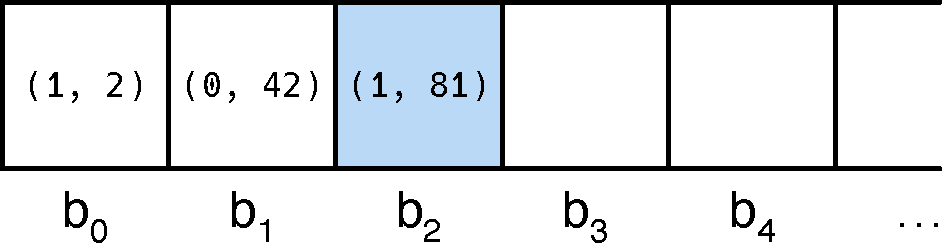
\includegraphics[width=\textwidth]{figs/sec3-1.pdf}
\end{minipage}
\label{sec:problem:loststate}
\item 
\begin{minipage}[b]{0.5\textwidth}
$[s_1 = \bot, s_2 = \bot, s_3 = \top, s_4 = \bot]$\\
(only the second log block is on disk) \\
\end{minipage}\quad%
\begin{minipage}{0.4\textwidth}
\vspace{-1.2em}
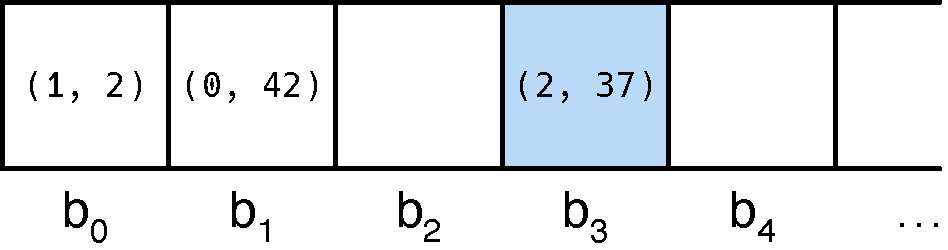
\includegraphics[width=\textwidth]{figs/sec3-2.pdf}
\end{minipage}

\item 
\begin{minipage}[b]{0.5\textwidth}
$[s_1 = \top, s_2 = \bot, s_3 = \top, s_4 = \bot]$\\
(both log blocks are on disk) \\
\end{minipage}\quad%
\begin{minipage}{0.4\textwidth}
\vspace{-1.2em}
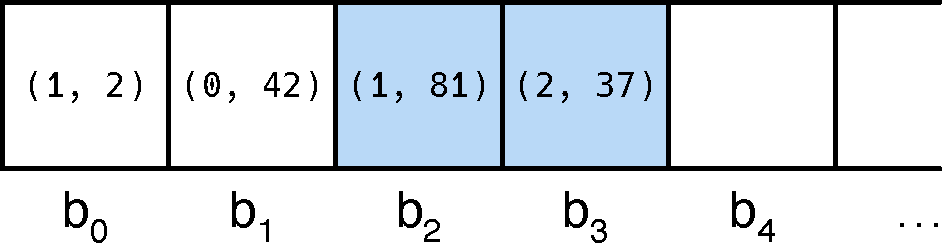
\includegraphics[width=\textwidth]{figs/sec3-3.pdf}
\end{minipage}

\item 
\begin{minipage}[b]{0.5\textwidth}
$[s_1 = \top, s_2 = \top, s_3 = \bot, s_4 = \bot]$\\
(the first log block and first superblock write are on disk)
\end{minipage}\quad%
\begin{minipage}{0.4\textwidth}
\vspace{-1.2em}
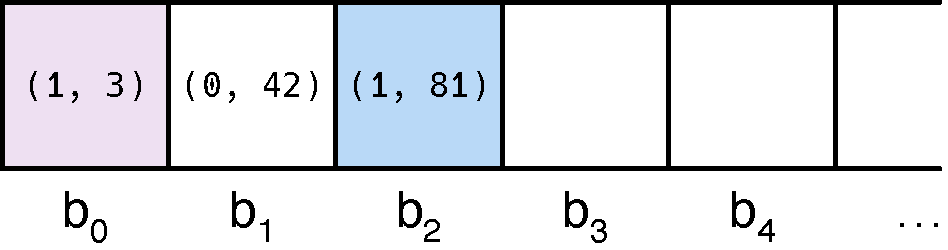
\includegraphics[width=\textwidth]{figs/sec3-4.pdf}
\end{minipage}

\item 
\begin{minipage}[b]{0.5\textwidth}
$[s_1 = \top, s_2 = \top, s_3 = \top, s_4 = \bot]$\\
(the first log block, first superblock write, and second log block are on disk)
\end{minipage}\quad%
\begin{minipage}{0.4\textwidth}
\vspace{-1.2em}
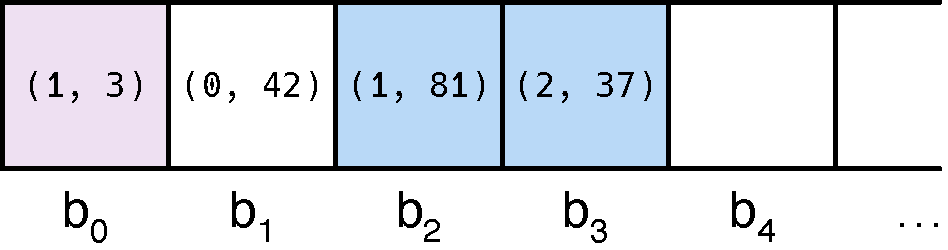
\includegraphics[width=\textwidth]{figs/sec3-5.pdf}
\end{minipage}
\end{enumerate}
%
Each of these states satisfies the key-value store's crash-consistency predicate $\consistent{d}$
defined in \cref{s:overview},
as in each case the superblock's \texttt{head} and \texttt{tail} pointers
refer only to log blocks that are also on disk.
Some states result in data loss after the crash---%
for example, neither key can be retrieved from crash state \ref{sec:problem:loststate} above, as the superblock is empty---%
but these states are still consistent
(i.e., they satisfy the log's representation invariant).
This set of two rules therefore makes the \texttt{SingleEntry_TwoAppend} litmus test crash consistent according to \cref{def:crash-consistent}.

If the second rule $\deprule{\textsf{superblock}}{\textsf{superblock}}{>}$ was excluded,
the rule set with one remaining rule allows 2 additional crash states:
%
\begin{enumerate}[resume,label={\raisebox{3\baselineskip}[0pt][0pt]{(\arabic*)}},ref=(\arabic*)]
\item 
\begin{minipage}[b]{0.5\textwidth}
$[s_1 = \top, s_2 = \bot, s_3 = \top, s_4 = \top]$\\
(the first log block, second log block, and second superblock write are on disk) \\
\end{minipage}\quad%
\begin{minipage}{0.4\textwidth}
\vspace{-4em}
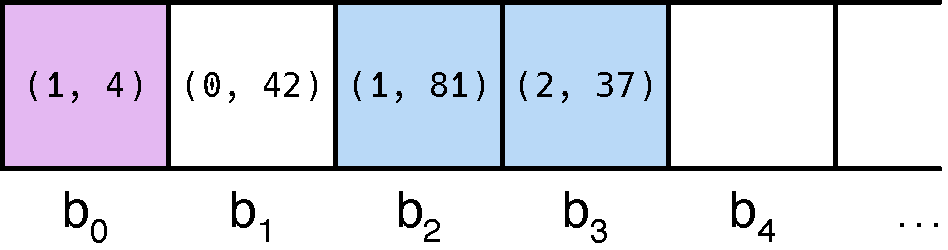
\includegraphics[width=\textwidth]{figs/sec3-6.pdf}
\end{minipage}
\label{sec:problem:goodstate}

\item 
\begin{minipage}[b]{0.5\textwidth}
$[s_1 = \bot, s_2 = \bot, s_3 = \top, s_4 = \top]$\\
(the second log block and second superblock write are on disk) \\
\end{minipage}\quad%
\begin{minipage}{0.4\textwidth}
\vspace{-4em}
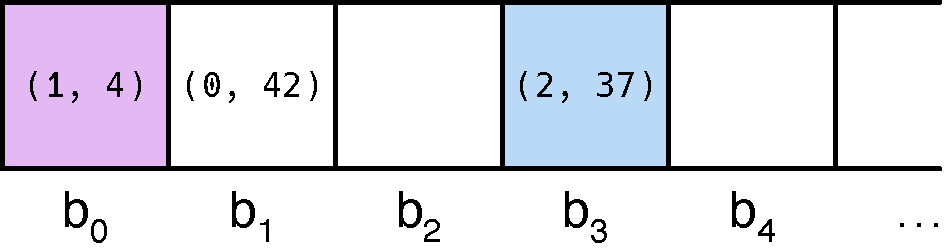
\includegraphics[width=\textwidth]{figs/sec3-7.pdf}
\end{minipage}
\label{sec:problem:badstate}
\end{enumerate}
%
\vspace{-1.5em}
State \ref{sec:problem:goodstate} satisfies the crash-consistency predicate despite losing the first superblock write,
as the second superblock write already contains the effects of the first one.
However, state \ref{sec:problem:badstate} violates the crash-consistency predicate:
the first log block is invalid,
but is included in the range between the superblock's \texttt{head} and \texttt{tail} pointers.
The set containing only the first rule therefore does not make \texttt{SingleEntry_TwoAppend} crash consistent.
\end{example}
